%%%%%%%%%%%%%%%%%%%%%%%%%%%%%%%%%%%%%%%%%%%%%%%%%%%%%%%%%%%%%%%%%%%%%%%
% Universidade Federal de Santa Catarina             
% Departamento de Automação e Sistemas                    
%                                                       
%
%%%%%%%%%%%%%%%%%%%%%%%%%%%%%%%%%%%%%%%%%%%%%%%%%%%%%%%%%%%%%%%%%%%%%%%
\documentclass [12pt, a4paper] {article}

\usepackage{float}
\usepackage[utf8]{inputenc}
\usepackage[brazil]{varioref}
\usepackage{graphicx,epsfig,psfrag}
\usepackage{gensymb}
\usepackage{amssymb}
\usepackage{mathtools}
\usepackage{amsmath}
\usepackage[english,brazil]{babel}
\usepackage{indentfirst}
\usepackage{float}
\usepackage{color}
\usepackage{listings}
\graphicspath{{./fig/}}
\definecolor{dkgreen}{rgb}{0,0.6,0}
\definecolor{gray}{rgb}{0.5,0.5,0.5}
\definecolor{mauve}{rgb}{0.58,0,0.82}
\lstset{frame=tb,
  language=Python,
  aboveskip=3mm,
  belowskip=3mm,
  showstringspaces=false,
  columns=flexible,
  basicstyle={\small\ttfamily},
  numbers=none,
  numberstyle=\tiny\color{gray},
  keywordstyle=\color{blue},
  commentstyle=\color{dkgreen},
  stringstyle=\color{mauve},
  breaklines=true,
  breakatwhitespace=true,
  tabsize=3
}

%\usepackage{etoolbox}
%\patchcmd{\thebibliography}{\chapter*}{\section}{}{}
%%%%%%%%%%%%%%%%%%%%%%%%%%%%%%%%%%%%%%%%%%%%%%%%%%%%%%%%%%%%%%%%%%%%%%%%
\begin{document}

\begin{titlepage}


%%%%%%%%%%%%%%%%%%%%%%%%%%%%%%%%%%%%%%%%%%%%%%%%%%%%%%%%%%%%%%%%%%%%%%%%
%   ____                  
%  / ___|__ _ _ __   __ _ 
% | |   / _` | '_ \ / _` |
% | |__| (_| | |_) | (_| |
%  \____\__,_| .__/ \__,_|
%            |_|          


	\centering
	{\Large Universidade Federal de Santa Catarina \par}
    {\Large DAS - Departamento de Automação e Sistemas \par}
	{\Large DAS410058 - Aprendizado de Máquina \par}
	\vspace{4cm}
	{\Huge\bfseries Trabalho Prático\par}
	\vspace{0.5cm}
	{\bfseries {\huge Aprendizado Indutivo}\par}
	%{\scshape\Large Escolha do projeto\par}
	\vspace{4cm}
	\emph{Alunos}\par
	{\large Alex Amadeu Cani \par}
    {\large Iago de Oliveira Silvestre\par}
	{\large Luis Felipe Pelison\par}

	\vspace{1.3cm}
	\emph{Professores}\par
	{\large Jomi F. Hubner \par}
    {\large  Marcelo Stemmer\par}
	

	\vfill
% Bottom of the page
	{\large Outubro de 2017\par}
\end{titlepage}
\tableofcontents

\newpage





















\section{Introdução}

O seguinte trabalho foi destinado à classificar páginas de universidades americanas entre alguns segmentos das próprias universidades. Essa tarefa, explicada no capítulo 2, incluiu a realização de uma pesquisa bibliográfica na área de aprendizado de máquina e ciência de dados (presente no capítulo 3), além de a implementação da solução, cuja requeriu os passos definidos pela metodologia CRISP-DM (capítulo 4). No fim, realizou-se uma coleta dos resultados obtidos (capítulo 5) e depois uma reflexão sobre as conclusões do trabalho (capítulo 6).
Todo o processo de programação desenvolvido pelo grupo está disponível no site: $https://github.com/lfpelison/ufsc-machinelearning-DAS410058/$









\section{Problema}

O problema é classificar páginas web de conteúdo acadêmico como sendo dos seguintes tipos:
\begin{itemize}
    \item de uma universidade
    \item de um departamento
    \item de um membro da faculdade
    \item de um projeto
    \item de um curso
    \item de um estudante
    \item ou outro tipo
\end{itemize}

Para isso iremos treinar um agente a classificar páginas web a partir de exemplos já classificados por um especialista humano. 
Os exemplos de páginas podem ser obtidos em $http://www.cs.cmu.edu/afs/cs.cmu.edu/project/theo-20/www/data/webkb-data.gtar.gz$ e estão organizados em diretórios que indicam a classificação. Por exemplo, a pasta $"student/cornell”$ contém páginas de alunos da universidade $Cornell$. 
A partir deste exemplos, iremos avaliar a qualidade de algumas técnicas/algoritmos de classificação.



















\section{Revisão Bibliográfica}









\subsection{CRISP-DM}

A sigla em inglês significa \textit{Cross Industry Standard Process for Data Mining}. Em português, podemos chamar de Processo Padrão Inter-Indústrias para Mineração de Dados. Pelo nome fica fácil identificar que o CRISP-DM é um padrão a ser seguido para a tarefa de \textit{Data Mining}. Esse padrão ou metodologia, é definido por \cite{crisp2} como um processo que descreve as principais decisões que os experientes mineradores de dados utilizam em seus trabalhos. E, de acordo com \cite{crisp}, o processo de mineração de dados possui 6 fases: Entendimento do negócio/problema, Entendimento dos dados, Preparação dos dados, Aplicação do modelo (Aprendizado de Máquina),
Análise e avaliação dos resultados e, por último, a produção.






\subsection{Aprendizado Supervisionado}

De acordo com \cite{am} e \cite{mohri}, os algoritmos de aprendizado de máquina podem ser organizados de acordo com diferentes critérios. Um deles diz respeito ao paradigma de aprendizado a ser adotada para lidar com a tarefa. De acordo com esse critério, as tarefas podem ser dividas em Preditivas e Descritivas. O aprendizado Supervisionado está dentro das tarefas Preditivas. Essas tarefas visam encontrar um valor desconhecido com base em um treinamento supervisionado, ou seja, um treinamento com a resposta dada por um "supervisor externo".







\subsection{CountVectorizer}

Um processo de limpeza e manipulação de dados muito importante para \textit{Text Mining} ou \textit{NLP} é o \textit{CountVectorizer}. De acordo com \cite{nlp}, esse processo é chamado de \textit{“vectorization and tokenization”}, em inglês, e pedaços do texto tornam-se \textit{tokens}. Se duas palavras são iguais, então o valor desse \textit{token} é 2. Se o valor de um \textit{token} for muito alto, considerado redundante, essa palavra é removida. Assim, tem-se uma tabela gigante, com o vocabulário dos dados, contendo todos os \textit{tokens}, e a quantidade de vezes que eles aparecem em cada documento. 


\subsection{Regressão Logística}

A regressão logística é um algoritmo de classificação que utiliza elementos estatísticos, como regressão, para fazer a predição de classes. De acordo com \cite{stat}, o modelo de regressão logística estima a probabilidade que uma característica pertence ou não aos dados (estima o sucesso), dadas as variáveis explicativas.

Na figura abaixo, retirada de \newline $http://www.cs.cmu.edu/afs/cs/usr/kdeng/www/thesis/logistic.pdf$
\newline
podemos ver um exemplo onde a regressão pode nos ajudar a classificar os pontos mais a esquerda, dos mais a direita.

\begin{figure}[!hbt]
		\begin{center}
		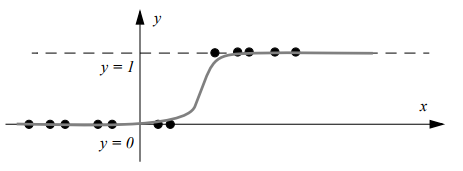
\includegraphics[width=1\columnwidth]{figuras/reglog.png}
		\end{center}
\end{figure}




\subsection{Florestas Randômicas}

As florestas randômicas partem da ideia dos algoritmos baseados em árvore. Esses algoritmos em árvore surgiram de \cite{quinlan}, em 1993. Neles, o espaço de entrada é particionado em pequenos segmentos, naqueles atributos que mais conseguem chegar em uma resposta para a classe alvo. Porém, essas árvores tradicionais ainda têm sérios problemas de \textit{overfitting}. Baseado nas primeiras árvores de decisão, as árvores randômicas são uma combinação de árvores de decisão tal que, cada árvore depende do valor de um vetor randômico para selecionar os atributos 'galhos', de acordo com \cite{random}. Esse método foi criado por \cite{forest} em 2001, e é na verdade um conjunto de classificadores mais fracos, que juntos formam um dos melhores algoritmos de classificação da atualidade.


\section{Solução}

Na solução do problema proposto na disciplina de Aprendizado de Máquina da Universidade Federal de Santa Catarina, o grupo realizou primeiramente um pré-processamento de dados, a fim de organizar os dados para uma melhor manipulação destes, dentro de um ambiente $Python$, em vez de trabalhar com os arquivos dentro de pastas, como foram disponibilizados. Após esse processo, de organização do conteúdo, realizou-se o processo conhecido na literatura como $CRISP-DM$. Nele, foram estudados os dados, entendidos e visualizados. Após essas etapas, preparamos os dados para inserir os algoritmos de aprendizado de máquina. Feito o aprendizado, as técnicas foram avaliadas e os resultados obtidos pelo grupo. Foram utilizados na solução algumas das principais técnicas de aprendizado de máquina, dentre elas: $Naive Bayes$, $Regressão Logística$, $Florestas Randômicas$ e $Gradient Boosting$. As tecnologias utilizadas foram a linguagem de programação $Python 2.7$, as \textit{notebooks} $jupyter-notebook$ e algumas bibliotecas $Python$ para ciência de dados: $Numpy$, $Pandas$, $scikit-learn$, $seaborn$ e $matplotlib$. Vale ressaltar que todo o código encontra-se no \textit{GitHub}: $https://github.com/lfpelison/ufsc-machinelearning-DAS410058/$



















\subsection{Pré-processamento de dados}

Inicialmente, os dados foram disponibilizados em diretórios. Cada diretório representa uma classe - o atributo saída da classificação, que queremos saber no final. Dentro desses diretórios, existem outras pastas, agora referentes a qual universidade pertencem. E, dentro dessas pastas das universidades, estão os arquivos html dos \textit{websites}.

Portanto, para realizar a manipulação desses dados, iremos transformar toda essa estrutura de diretórios para um arquivo $.csv$, que contenha 4 atributos: 
\begin{itemize}
\item url - endereço do site
\item html - conteúdo do site
\item university - universidade pertencente
\item target - classificação do site (pode ser de um aluno, professor, ...)
\end{itemize}

O atributo mais importante para nós, será o html da página. Será a partir dele que tentaremos classificar o site. Por tanto, para recuperar esse conteúdo html, processamos todos os arquivos, entrando em cada pasta da base de dados, e coletamos o texto que está dentro dos limites de $<html>$ e $</html>$. Isso foi realizado com um script $Python$ abaixo, que cria um arquivo chamado $corpus.csv$ contendo a estrutura dos 4 atributos que queríamos. \\


\begin{lstlisting}
urls = []
for dirpath, dirnames, filenames in os.walk("./webkb"):
    for filename in filenames:
        urls.append(os.path.join(dirpath, filename))
print len(urls)
regex = r"\<([\s\S]*)>"
with open('corpus.csv', 'w') as output:
    for j, i in enumerate(urls):
        with open(i) as input:
            if j == 0:
                output.write("url-||-university-||-html-||-target \n")
            search = re.search(regex, input.read())
            if search: 
                html = search.group(0).replace('\n', ' ').replace('\r', '')
            else:
                html = 'NaN'
            target = i.split("/")[2]
            university = i.split("/")[3]
            url = i.split("/")[4]
            print j
            output.write("{0}-||-{1}-||-{2}-||-{3} \n".format(url, university, html, target))
\end{lstlisting}

Com o arquivo $.csv$, o tratamento dos dados fica muito mais fácil. 

A próxima etapa agora é passar esse arquivo para o formato de uma tabela. Agindo nesse sentido, utilizaremos a biblioteca $Pandas$ que é a mais apropriada em $Python$ para trabalhar com dados tabulares de maneira eficiente. 


\begin{lstlisting}
path = './corpus.csv'
one = pd.read_csv(path, sep=r"\-\|\|-", quotechar='"', engine='python')
\end{lstlisting}
\newpage


\subsection{Entendendo e manipulando os dados}

Seguindo para a utilização da metodologia $CRISP-DM$, com os dados organizados no $Pandas$, podemos visualizar algumas informações sobre eles.

Primeiramente, verificamos se todos os dados do conjunto de dados inicial foi passado de forma integral ao $Pandas$. Com os comandos $one.head()$ e $one.describe()$ podemos ver isso, além de visualizar algumas linhas da tabela. A execução desses 2 comandos, nos resultou na seguinte Figura:


\begin{figure}[!hbt]
		\begin{center}
		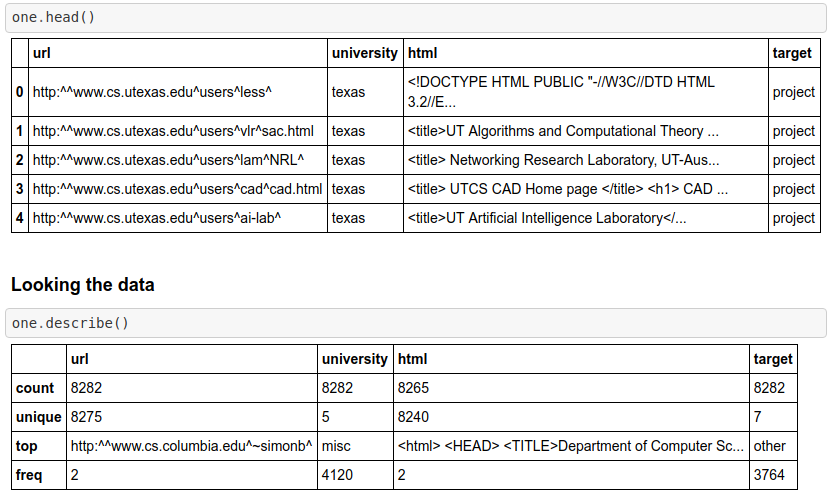
\includegraphics[width=1\columnwidth]{figuras/1.png}
		\end{center}
\end{figure}

Dessa figura podemos ter certeza que os 8282 dados foram importados corretamente. Também, a estrutura dos atributos, definidas anteriormente, foi respeitada. Podemos até mesmo ver os 5 primeiros dados da tabela.

Com essas informações, também temos um entendimento do problema como um todo, que será a classificação das páginas das universidades. Iremos utilizar o conteúdo html para classificação se a página é do professor, do aluno, do departamento, entre outras possibilidades. Essas possibilidades podem ser visualizadas com o comando $one.groupby(one['target']).count()$. Que também nos possibilita conferir se o número desses dados corresponde com o passado pela base de dados $webkb$.
Então, a Figura abaixo, nos mostra que sim, todos os dados estão presentes, além das classes possíveis.

\newpage

\begin{figure}[!hbt]
		\begin{center}
		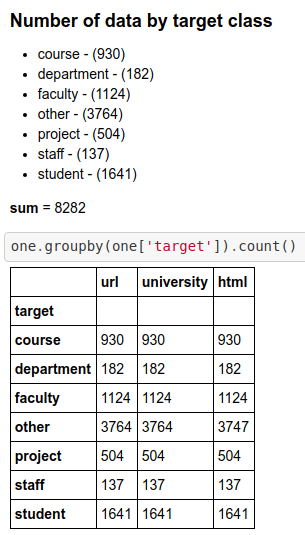
\includegraphics[width=0.6\columnwidth]{figuras/classes.png}
		\end{center}
\end{figure}


Ainda nos resta verificar se existem dados nulos nessa tabela. Para isso, aplicaremos os seguintes comandos:

\begin{lstlisting}
# Who is 'Nan'?
one[one['html'].isnull()]

# Deleting rows with null values. There are 17 rows.
one = one.dropna(axis=0, how='any')
\end{lstlisting}

Com isso, acabamos de apagar os dados que continham htmls vazios. No total, 17 linhas foram apagadas da base de dados. Como tínhamos 8282 dados, 17 não representam muita coisa para nós. Agora temos 8265 dados.












\subsection{Visualização dos Dados}

Uma das principais partes da metodologia $CRISP-DM$ é entender bem os dados e o problema que estamos lidando. Essa etapa é essencial no processo de ciência de dados, a chamada visualização de dados. Com ela podemos ter um melhor entendimento de como nossa base de dados está preenchida.

Começamos, então, plotando alguns gráficos que nos mostram a quantidade de dados que temos, divididos por universidades.

\begin{figure}[!hbt]
		\begin{center}
		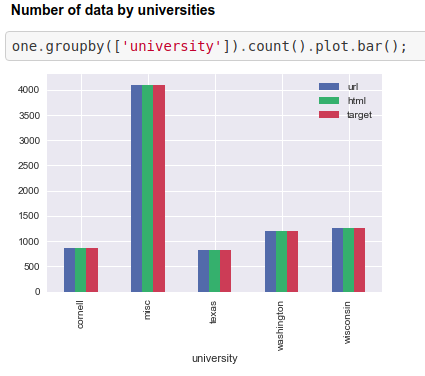
\includegraphics[width=1\columnwidth]{figuras/universidades.png}
		\end{center}
\end{figure}

Podemos perceber que existem muitos dados $MISC$, que representam várias universidades juntas. Isso não é tão bom, pois não temos informações exatas sobre as universidades que compõe o $MISC$, e também pois a base é desbalanceada, já que existe a predominância de um atributo. Porém, isso não nos afeta tanto, já que não queremos predizer a qual universidade os dados pertencem.

Outra informação que podemos tirar dessa figura é que as duas universidades que possuem mais dados, são $Washington$ e $Wisconsin$. Essas, serão utilizadas depois para um treinamento individual e teste em outra. A fim de provar a acurácia de nossas classificações.


Depois, os dados foram agrupados pela classe.

\begin{figure}[!hbt]
		\begin{center}
		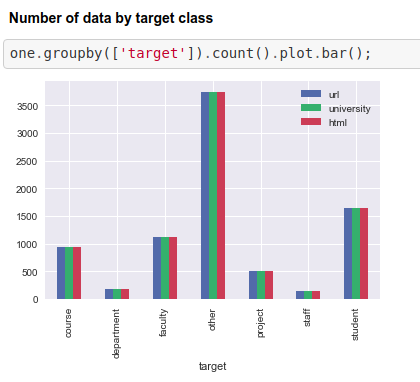
\includegraphics[width=1\columnwidth]{figuras/target.png}
		\end{center}
\end{figure}

Aqui, podemos verificar novamente um desbalanceamento de atributo, pois $Other$ domina as outras. Agora sim isso é um problema para nós, já que qualquer algoritmo de classificação tenderá a escolher $Other$ como resposta da predição, já que ela é a mais provável, devido ao número de vezes que aparece no conjunto de dados. Poderíamos retirar uma parte, para a classificação ficar mais justa. Porém, como queremos analisar todo o conjunto, iremos deixá-la.

E, por fim, uma visão geral pode ser obtida com um gráfico que mostra os dois.

\begin{figure}[!hbt]
		\begin{center}
		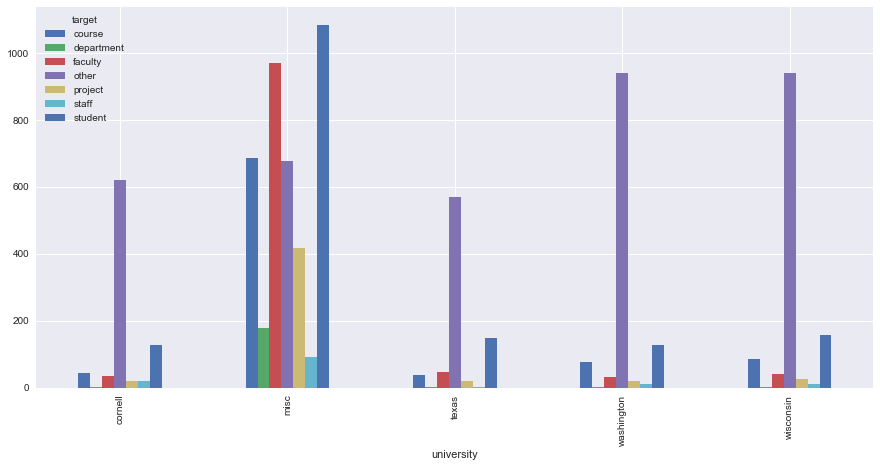
\includegraphics[width=1\columnwidth]{figuras/dados.png}
		\end{center}
\end{figure}

De novo, surgem como destoantes as classes $Misc$ e $Other$. Porém, iremos manter os dados da forma que vieram. Não faremos a exclusão de mais dados, além dos nulos.














\subsection{Seleção dos atributos}

Para classificarmos as páginas web, iremos utilizar a classe $Target$ do conjunto de dados como fim. Essa classe, pode ser:

\begin{itemize}
\item course - página de um curso
\item department - página de um departamento
\item faculty	- página de uma faculdade
\item other - página qualquer da universidade
\item project	- página de um projeto
\item staff - página de um administrador da universidade
\item student	- página de um estudante
\end{itemize}

Porém, iremos deixar mais fácil para os algoritmos. Trocaremos as classes simbólicas para números. Assim, mapearemos da seguinte forma a nova classe $Target\_num$:

\begin{lstlisting}
one['target_num'] = one.target.map({'course':0, 'department':1, 'faculty':2, 'other':3, 'project':4, 'staff':5, 'student':6})
\end{lstlisting}


Com isso feito, formalmente esclareceremos quem será o atributo a ser classificado (aprendizado supervisionado) e quem serão os atributos que serão levados em conta.

\begin{lstlisting}
X = one.html
y = one.target_num
\end{lstlisting}

Escolhemos somente o html como dado a ser levado em conta para a classificação do target, porém, poderíamos também colocar a url, já que é uma informação que nós temos. Essa ideia fica para um estudo futuro desse problema.


Na sequência, iremos separar o conjunto de dados em teste e treino. Escolhemos uma taxa de 25\% para teste e 75\% para treino. 

\begin{lstlisting}
# split X and y into training and testing sets

from sklearn.model_selection import train_test_split


X_train, X_test, y_train, y_test = train_test_split(X, y, random_state=1)
print(X_train.shape)
print(X_test.shape)
print(y_train.shape)
print(y_test.shape)
\end{lstlisting}

A última etapa na escolha dos atributos, e a mais importante delas para a solução do problema, é a realização do $CountVectorizer$. Essa técnica realiza a contagem de palavras de todos os dados de treino. Ela "entra" em cada html, dos dados de treino, procura por todas as palavras e conta quantas existem para cada dado. Assim, existe um vocabulário de palavras para todos os documentos. E, cada documento possui seu conjunto de palavras e o número de vezes que cada uma apareceu. Assim, todos os documentos (ou linhas da tabela, se preferir), possuirá como atributos todas as palavras do vocabulário feito pelo $CountVectorizer$. E, a quantidade de cada palavra irá compor os dados desses atributos. 
Assim, os atributos que serão levados em conta para a classificação da classe target, serão a quantidade de palavras, do vocabulário, presentes no html de cada página.

Entendido esse processo, iremos colocar os dados de teste no mesmo formato dos dados de treino, com o mesmo vocabulário. É importante notar que, nessa parte, não realizamos a adição de novas palavras no vocabulário, pois os arquivos de teste não devem interferir nisso, são exatamente, conjuntos de testes, que servirão como páginas nunca antes vistas pelos algoritmos.

Outra importante notificação aqui, diz respeito aos parâmetros passados ao $CountVectorizer$. Um dos parâmetros, o $n-gram$ é muito importante, já que ele define a possibilidade de formar palavras compostas. No nosso caso, o $n-gram$ vale 2, assim, podemos ter palavras compostas, e não somente palavras únicas no html, como: $"hello \;\ student"$ e não somente $"hello"$ ou $"student"$. 

O código que realiza essa parte é o seguinte:

\begin{lstlisting}
from sklearn.feature_extraction.text import CountVectorizer
#from sklearn.feature_extraction.text import TfidfVectorizer

# instantiate the vectorizer

vect = CountVectorizer(encoding='latin-1', stop_words='english', ngram_range=(1, 2), min_df=5)
#vect = TfidfVectorizer(encoding='latin-1', stop_words='english', ngram_range=(1, 2), min_df=5)
# Esse tfIdf não funcionou muito bem

                       
# combine fit and transform into a single step

X_train_dtm = vect.fit_transform(X_train)
X_train_dtm


# transform testing data (using fitted vocabulary) into a document-term matrix

X_test_dtm = vect.transform(X_test)
X_test_dtm
\end{lstlisting}

Outros parâmetros utilizados foram a presença de $Stop Words$, que são palavras insignificantes para a semântica da classificação como: $a$, $the$, ...
e também o parâmetro $min\_df = 5$, que significa a inclusão de palavras no vocabulário que aparecem no mínimo em 5 itens dos 6198 treinados.

Outra observação é que no código existe a utilização do $TfIDF$, porém comentada. Essa técnica é bem interessante, porém com base em testes realizados, não chegamos em resultados melhores utilizando-a. Portanto, deixaremos de fora da explicação aqui, já que não foi utilizada de fato para a solução do problema.



\subsection{Aplicação dos modelos de aprendizado}


Com os dados prontos, resta a aplicação dos algoritmos de aprendizado.
Para esse problema, iremos aplicar alguns algoritmos vistos na disciplina e outros mais sofisticados. Eles são facilmente aplicados com a biblioteca $sklearn$, para o $Python$. Com poucas linhas de código, alinhamos nossos dados e conseguimos predizer a classe alvo.

Basicamente, todos os algoritmos têm uma sequência básica de passos. Esses passos são o $fit$, que aprende, de acordo com seu modelo, quais os valores de X que geram Y. E, o $predict$, que pega novos dados, e tenta acertar quais serão as saídas para eles, de acordo com o modelo aprendido no $fit$. O último passo é verificar o quão bem esse modelo foi. Medindo a quantidade de acertos que fez.

O primeiro modelo que realizamos foi o algoritmo de $Regressão \;\ Logística$. Um modelo que utiliza regressão para fazer a classificação. Explicado no capítulo de revisão bibliográfica.

\begin{lstlisting}
# import and instantiate a logistic regression model

from sklearn.linear_model import LogisticRegression
logreg = LogisticRegression(class_weight='balanced')

# train the model using X_train_dtm

logreg.fit(X_train_dtm, y_train)


# make class predictions for X_test_dtm

y_pred_class = logreg.predict(X_test_dtm)


# calculate accuracy
from sklearn import metrics

metrics.accuracy_score(y_test, y_pred_class)
\end{lstlisting}

Como resultado, obtivemos incríveis $83.50\%$. Um valor bem alto de acertos para dados bem crus.


Depois, utilizamos o modelo de $Árvores \;\ Randômicas$. Muito conhecido por acertar muitas classificações. Também foi explicado na revisão bibliográfica. 

\begin{lstlisting}

from sklearn.ensemble import RandomForestClassifier
forest = RandomForestClassifier(n_estimators=300)

forest.fit(X_train_dtm, y_train)


y_pred_class = forest.predict(X_test_dtm)

metrics.accuracy_score(y_test, y_pred_class)

\end{lstlisting}

Com ele obtivemos $81.08\%$ de acurácia. Um grande valor também, porém menor que o de regressão logística.

Para simples verificação de outros modelos, realizamos o aprendizado com $Naive \;\ Bayes$ e com o $Gradiente \;\ Boosting$, algoritmos que não foram citados na revisão bibliográficas, mas pela facilidade da biblioteca $sklearn$ nós resolvemos verificar o quão bem eles classificavam.

\begin{lstlisting}

# import and instantiate a Multinomial Naive Bayes model

from sklearn.naive_bayes import MultinomialNB
nb = MultinomialNB()

# train the model using X_train_dtm (timing it with an IPython "magic command")

nb.fit(X_train_dtm, y_train)

# make class predictions for X_test_dtm

y_pred_class = nb.predict(X_test_dtm)


# calculate accuracy of class predictions

from sklearn import metrics
metrics.accuracy_score(y_test, y_pred_class)

\end{lstlisting}

Com $Bayes$, um modelo probabilístico, obtivemos apenas $60.32\%$ de acurácia.

\begin{lstlisting}

from sklearn.ensemble import GradientBoostingClassifier
clf = GradientBoostingClassifier(n_estimators=100,learning_rate=1.0,max_depth=1,random_state=0)

clf.fit(X_train_dtm, y_train)

X_test_array = X_test_dtm.toarray()

y_pred_class = clf.predict(X_test_array)

metrics.accuracy_score(y_test, y_pred_class)

\end{lstlisting}

Já, com o $Gradient Boosting$, obtivemos $78.64\%$ de acurácia.



\subsection{Extra}


A fim de certificar a grande acurácia que obtivemos com o algoritmo de Regressão Logística obtido nos dados completos, realizamos um estudo contendo apenas dados de teste da universidade de $Wisconsin$. Com os dados dessa universidade, procuraremos testar as páginas de web da universidade de $Washington$. Assim, se a acurácia continuar alta, o nosso modelo de aprendizado foi bem sucedido.

Para isso, realizamos o seguinte código:

\begin{lstlisting}

washington = one[one.university == 'washington']
wisconsin = one[one.university == 'wisconsin']


# Define X and y (from the data) for use with COUNTVECTORIZER

#Training data

X_wisconsin = wisconsin.html
y_wisconsin = wisconsin.target_num


#Testing data

X_washington = washington.html
y_washington = washington.target_num

---------------------------------------------------------------

from sklearn.feature_extraction.text import CountVectorizer
#from sklearn.feature_extraction.text import TfidfVectorizer

# instantiate the vectorizer

vect = CountVectorizer(encoding='latin-1', stop_words='english', ngram_range=(1, 2), min_df=5)
#vect = TfidfVectorizer(encoding='latin-1', stop_words='english', ngram_range=(1, 2), min_df=5)
# Esse tfIdf deu ruim

                       
# combine fit and transform into a single step

X_wisconsin_dtm = vect.fit_transform(X_wisconsin)
X_wisconsin_dtm


# transform testing data (using fitted vocabulary) into a document-term matrix

X_washington_dtm = vect.transform(X_washington)
X_washington_dtm

\end{lstlisting}

E, aplicamos novamente o $Random \;\ Forest$.

\begin{lstlisting}
from sklearn.ensemble import RandomForestClassifier
from sklearn import metrics

forest = RandomForestClassifier(n_estimators=300)

%time forest.fit(X_wisconsin_dtm, y_wisconsin)

y_pred_washington = forest.predict(X_washington_dtm)

metrics.accuracy_score(y_washington, y_pred_washington)
\end{lstlisting}

Que nos resultou em uma acurácia de $78.50\%$.


\section{Resultados}

Para facilitar a leitura, colocamos a acurácia de cada algoritmo logo depois de seus códigos, no capítulo anterior. Portanto, aqui haverá uma repetição dos valores do capítulo 4, porém com alguns comentário a mais.

O mais impactante resultado obtido foi a taxa de acerto da regressão logística. Ela nos deu uma acurácia superior a $83\%$ o que satisfez os integrantes do grupo. Pois, o nosso processamento dos dados foi muito pequeno. Apenas excluímos alguns textos dos arquivos, deixando tudo que estava entre as \textit{tags} $<html>$, e alguns htmls nulos. Portanto, o resultado agradou e nada além do $CountVectorizer$, com $n-gram$, foi realizado.














\subsection{Comparativo em taxa de acerto}
No quesito de acertos do algoritmo, quem apresentou a maior taxa foi o algoritmo de \textit{Logistic Regression} com 83,5\%, seguido de \textit{Random Forest} com 81,0\%, \textit{Gradient Boosting} com 1min e 78,6\% e por fim o algoritmo com pior taxa de acerto foi \textit{Naive Bayes} com 60,3\%.

\subsection{Comparativo em tempo computacional}
No quesito de tempo gasto realizando o algoritmo, quem apresentou o menor tempo computacional foi o algoritmo de \textit{Naive Bayes} com 63ms, seguido de \textit{Gradient Boosting} com 59s, \textit{Random Forest} com 1min e 20s e por fim o mais lento foi \textit{Logistic Regression} com tempo total de 1min 26s.



















\section{Conclusão}

Com os dados sem muito pré-processamento, somente a integração destes em um arquivo $.csv$, depois a técnica $CountVectorizer$, com parâmetros de $n-gram$ e $min\_df$ bem definidos, pudemos obter uma taxa altíssima de acertos com 2 algoritmos classificadores de aprendizado supervisionado de máquina: $Regressão \;\ Logística$ e $Árvores \;\ Randômicas$. Esse sucesso foi bem recebido pelos integrantes, que a priori tinham pensado que o trabalho de processamento dos dados seria intenso. Porém, logo de cara, mostrou-se que não. Então, a principal conclusão desse trabalho foi de que com o mínimo de processamento, devemos testar os algoritmos de aprendizado, a fim de verificar se uma alta taxa de acertos já é obtida. Outras conclusões são de que a linguagem $Python$ com suas bibliotecas para análise de dados facilitam muito a vida de cientistas de dados que manipulam bases e testam algoritmos de aprendizado de máquina. No fim, o problema foi solucionado com alta taxa de acerto, tanto para a base de dados toda, quanto para apenas uma universidade servindo de treino para outra universidade. Quanto aos algoritmos, mostrou-se que um algoritmo simples de regressão pode vencer outros mais complexos, como as árvores randômicas e principalmente o \textit{Gradient Boosting}, um algoritmo mais recente e poderoso de aprendizado de máquina.

\newpage

\begin{thebibliography}{1}

  \bibitem{crisp} C. Shearer, “The CRISP-DM model: the new blueprint for data mining,” Journal of Data Warehousing, vol. 5, pp. 13-22, 2000

  \bibitem{crisp2}  Pete Chapman, Julian Clinton , Randy Kerber et al, “The CRISP-DM User Guide”, 1999 

  \bibitem{mohri} M. Mohri, A. Rostamizadeh, and A. Talwalkar, Foundations of
Machine Learning. MIT Press, 2012.

  \bibitem{am} FACELI, Katti; LORENA, Ana Carolina; GAMA, João; CARVALHO, André Carlos Ponce de Leon Ferreira de. Inteligência artificial: uma abordagem de aprendizado de máquina, 2011.
  
  \bibitem{nlp} Using Machine Learning and Natural Language Processing Algorithms to Automate the Evaluation of Clinical Decision Support in Electronic Medical Record Systems. Donald A Szlosek, MPHi and Jonathan Ferrettii
  
  \bibitem{stat} T. Hastie, R. Tibshirani, J. Friedman, The Elements of Statistical Learning, Springer-Verlag, New York, 2001.
  
  \bibitem{quinlan} Quinlan, J.R. Mach Learn (1986) 1: 81. https://doi.org/10.1007/BF00116251
  
  \bibitem{random} Breiman, L. Machine Learning (2001) 45: 5. https://doi.org/10.1023/A:1010933404324
  
  \bibitem{forest} Leo Breiman. 2001. Random Forests. Mach. Learn. 45, 1 (October 2001), 5-32. DOI: https://doi.org/10.1023/A:1010933404324

    
\end{thebibliography}



\end{document}


















